\documentclass{article}\usepackage[]{graphicx}\usepackage[]{color}
%% maxwidth is the original width if it is less than linewidth
%% otherwise use linewidth (to make sure the graphics do not exceed the margin)
\makeatletter
\def\maxwidth{ %
  \ifdim\Gin@nat@width>\linewidth
    \linewidth
  \else
    \Gin@nat@width
  \fi
}
\makeatother

\definecolor{fgcolor}{rgb}{0.345, 0.345, 0.345}
\newcommand{\hlnum}[1]{\textcolor[rgb]{0.686,0.059,0.569}{#1}}%
\newcommand{\hlstr}[1]{\textcolor[rgb]{0.192,0.494,0.8}{#1}}%
\newcommand{\hlcom}[1]{\textcolor[rgb]{0.678,0.584,0.686}{\textit{#1}}}%
\newcommand{\hlopt}[1]{\textcolor[rgb]{0,0,0}{#1}}%
\newcommand{\hlstd}[1]{\textcolor[rgb]{0.345,0.345,0.345}{#1}}%
\newcommand{\hlkwa}[1]{\textcolor[rgb]{0.161,0.373,0.58}{\textbf{#1}}}%
\newcommand{\hlkwb}[1]{\textcolor[rgb]{0.69,0.353,0.396}{#1}}%
\newcommand{\hlkwc}[1]{\textcolor[rgb]{0.333,0.667,0.333}{#1}}%
\newcommand{\hlkwd}[1]{\textcolor[rgb]{0.737,0.353,0.396}{\textbf{#1}}}%

\usepackage{framed}
\makeatletter
\newenvironment{kframe}{%
 \def\at@end@of@kframe{}%
 \ifinner\ifhmode%
  \def\at@end@of@kframe{\end{minipage}}%
  \begin{minipage}{\columnwidth}%
 \fi\fi%
 \def\FrameCommand##1{\hskip\@totalleftmargin \hskip-\fboxsep
 \colorbox{shadecolor}{##1}\hskip-\fboxsep
     % There is no \\@totalrightmargin, so:
     \hskip-\linewidth \hskip-\@totalleftmargin \hskip\columnwidth}%
 \MakeFramed {\advance\hsize-\width
   \@totalleftmargin\z@ \linewidth\hsize
   \@setminipage}}%
 {\par\unskip\endMakeFramed%
 \at@end@of@kframe}
\makeatother

\definecolor{shadecolor}{rgb}{.97, .97, .97}
\definecolor{messagecolor}{rgb}{0, 0, 0}
\definecolor{warningcolor}{rgb}{1, 0, 1}
\definecolor{errorcolor}{rgb}{1, 0, 0}
\newenvironment{knitrout}{}{} % an empty environment to be redefined in TeX

\usepackage{alltt}
\usepackage[utf8]{inputenc}
\usepackage{amsmath}
\usepackage{amssymb}
\usepackage{float}
\newtheorem{theorem}{THEOREM}
\newtheorem{proof}{PROOF}
\usepackage{natbib}
\usepackage{graphicx}
\newcommand\inv[1]{#1\raisebox{1.15ex}{$\scriptscriptstyle-\!1$}}

\title{Simple Regression Analysis}
\author{YOUNG HOON KIM}
\date{Oct 31, 2016}
\IfFileExists{upquote.sty}{\usepackage{upquote}}{}
\begin{document}

\maketitle



\section*{Abstract} In this report, I am going to reproduce the main results displayed in Section 3.1 \emph{Simple Linear Regression} (Chapter 3) of the book \textbf{An Introduction to Statistical Learning}.

\section*{Introduction} The overall goal is to provide advice on how to improve sales of the particular product. More specifically, the idea is to determine whether there is an association between advertising and sales, and if so, develop an accurate model that can be used to predict sales on the basis of the three media budgets.  

\section*{Data} The Advertising data set consists of the \textbf{Sales} (in thousands of units) of a particular product in 200 different markets, along with advertising budgets (in thousands of dollars) for the product in each of those markets for three different media: \textbf{TV}, \textbf{Radio}, and \textbf{Newspaper}.

\section*{Methodology}
We consider one media from the data set, TV, and study its relationship with Sales. For this purpose, we use a simple linear model:
\begin{equation}
\centering
Sales= \beta_0 + \beta_1TV
\end{equation}
To estimate the coefficients $\beta_0$ and $\beta_1$ we fit a regression model via the least squares criterion.

\section*{Results}
We compute the regression coefficients  
\begin{knitrout}
\definecolor{shadecolor}{rgb}{0.969, 0.969, 0.969}\color{fgcolor}\begin{kframe}
\begin{verbatim}
## \begin{table}[!h]
## \centering
## \begin{tabular}{rrrrr}
##   \hline
##  & Estimate & Std. Error & t value & Pr($>$$|$t$|$) \\ 
##   \hline
## (Intercept) & 7.03 & 0.46 & 15.36 & 0.00 \\ 
##   tv & 0.05 & 0.00 & 17.67 & 0.00 \\ 
##    \hline
## \end{tabular}
## \end{table}
\end{verbatim}
\end{kframe}
\end{knitrout}

\begin{table}[!h]
\centering
\caption{Information about Regression Coefficients}
\begin{tabular}{rrrrr}
  \hline
 & Estimate & Std. Error & t value & Pr($>|t|$) \\ 
  \hline
(Intercept) & 7.03 & 0.46 & 15.36 & 0.00 \\ 
  tv & 0.05 & 0.00 & 17.67 & 0.00 \\ 
   \hline
\end{tabular}
\end{table}  
More information about the least squares model is given in the table below:  
\begin{table}[ht]
\centering
\begin{tabular}{rlr}
  \hline
 & Quantity & Value \\ 
  \hline
1 & RSE & 3.26 \\ 
  2 & R2 & 0.61 \\ 
  3 & F-stat & 312.14 \\ 
   \hline
\end{tabular}
\end{table}




\begin{figure}[!ht]
\centering
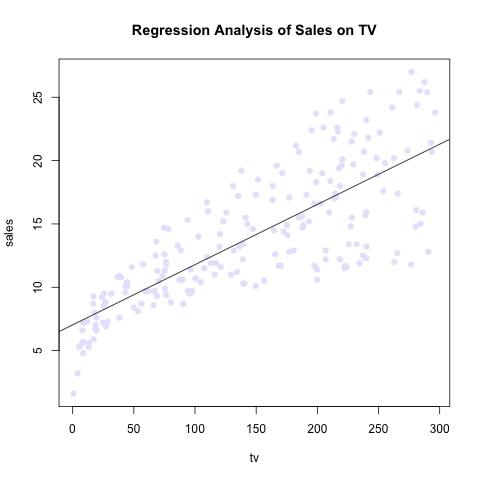
\includegraphics[width=10cm]{scatterplot-tv-sales.png}
\caption{Scatterplot with fitted regression line}
\end{figure}

Here is the scatterplot.

\section*{Conclusions}
That's it!

\end{document}
